\documentclass[12pt,aspectratio=169]{beamer}
\usetheme{metropolis}
\setbeamersize{text margin left=.5cm,text margin right=.5cm}
\usepackage[lf]{carlito}
\usepackage{siunitx}
\usepackage{tikz}
\usepackage{mathpazo}
\usepackage{bm}
\usepackage{mathtools}
\usepackage[ISO]{diffcoeff}
\diffdef{}{ op-symbol=\mathsf{d} }
\usepackage{xcolor,colortbl}

\setmonofont{Ubuntu Mono}
\setlength{\parskip}{0pt}
\renewcommand{\baselinestretch}{1}

\sisetup{
  inter-unit-product=\cdot,
  per-mode=symbol
}

\tikzset{
  >=latex
}

%\newcommand{\iii}{\hat{\bm\imath}}
%\newcommand{\jjj}{\hat{\bm\jmath}}
%\newcommand{\kkk}{\hat{\bm k}}

\usepackage[siunitx]{circuitikz} % to draw circuits!

\title{Topic 13: Magnetism}
\subtitle{Advanced Placement Physics C}
\author[TML]{Dr.\ Timothy Leung}
\institute{Olympiads School}
\date{Updated: Summer 2022}

\newcommand{\pic}[2]{
  \includegraphics[width=#1\textwidth]{#2}
}
\newcommand{\eq}[2]{
  \vspace{#1}{\Large
    \begin{displaymath}
      #2
    \end{displaymath}
  }
}
%\newcommand{\iii}{\ensuremath\hat{\bm{\imath}}}
%\newcommand{\jjj}{\ensuremath\hat{\bm{\jmath}}}
%\newcommand{\kkk}{\ensuremath\hat{\bm{k}}}
\newcommand{\iii}{\ensuremath\hat\imath}
\newcommand{\jjj}{\ensuremath\hat\jmath}
\newcommand{\kkk}{\ensuremath\hat k}


\begin{document}

\begin{frame}
  \maketitle
\end{frame}


\section{Magnetic Field}

\begin{frame}{Review of Magnetic Field}
  \begin{itemize}
  \item Magnetism is generated by moving charged particles, e.g.
    a single charge, or an electric current
  \item It can also be generated by permanent magnets, or Earth
  \end{itemize}
\end{frame}



\begin{frame}{Review of Magnetic Field}
  \begin{itemize}
  \item Magnetism affects other \emph{moving} charged particles
  \item The vector field is called the \textbf{magnetic field}
  \item Magnetic field has unit \textbf{tesla}
  \item Magnetic field lines have no ends---they always run in a loop
  \end{itemize}
\end{frame}



\begin{frame}{Magnetic Field Generated by a Moving Point Charge}
  \begin{center}
    \pic{.35}{pointchargeB}
  \end{center}
  A point charge generates an electric field $\vec E$. When it's moving, it
  also generates a magnetic field $\vec B$, given by the equation:

  \eq{-.2in}{
    \boxed{\vec B=\frac{\mu_0}{4\pi}\frac{q\vec v\times\hat r}{r^2}}
  }

  The direction of $\vec B$ can be obtained by applying the
  \emph{right hand rule} if you are not confident with cross products.
\end{frame}



\begin{frame}{Reminder on the cross product}
  Whenever the ``right hand rule'' is mentioned, or when an equation has
  ``$\sin\theta$'' in it, that usually means that the equation involces a
  cross product in it. Just a reminder on a few properties:
  \begin{itemize}
  \item If $\vec C=\vec A\times\vec B$, then $\vec C$ is perpendicular to both
    $\vec A$ and $\vec B$.
  \item The length of the cross product of two vectors is:
    
    \eq{-.25in}{
      |\vec A\times\vec B|=|\vec A||\vec B|\sin\theta
    }
    where $\theta$ is the angle between $\vec A$ and $\vec B$
  \item Cross products are anti-commutable:

    \eq{-.25in}{
      \vec A\times\vec B=-\vec B\times\vec A
    }
  \end{itemize}
\end{frame}



\begin{frame}{Magnetic Field Generated by a Moving Point Charge}

  \eq{-.05in}{
    \boxed{\vec B=\frac{\mu_0}{4\pi}\frac{q\vec v\times\hat r}{r^2}}
  }
  \begin{center}
    \begin{tabular}{l|c|c}
      \rowcolor{pink}
      \textbf{Quantity} & \textbf{Symbol} & \textbf{SI Unit} \\ \hline
      Magnetic field                  & $\vec B$ & \si\tesla \\
      Charge                          & $q$      & \si\coulomb \\
      Velocity of the charge          & $\vec v$ & \si{\meter\per\second}\\
      Distance from the moving charge & $r$      & \si\metre\\
      Radial outward unit vector from the charge & $\hat r$ & no units\\
      Permeability of free space & $\mu_0$ & \si{\tesla\metre\per\ampere}
    \end{tabular}
  \end{center}
  \textbf{Permeability of free space} (or \textbf{vacuum permeability}) is a
  constant with a value of
  $\mu_0=4\pi\times\num{e-7}\;\si{\tesla\metre\per\ampere}$. It measures how
  well a space can become magnetized.
\end{frame}



\begin{frame}{Biot-Savart Law}
  \begin{columns}
    \column{.25\textwidth}
    \pic1{bsav}
    
    \column{.75\textwidth}
    An electric current is really many charges particles moving along a wire;
    each charge creating its own magnetic field.
    The total magnetic field in the wire is the integral of the contribution
    ($\dl\vec B$) of the current ($I$) from each infinitesimal sections
    ($\dl\vec L$) of the wire, given by the \textbf{Biot-Savart law}:
  
    \eq{-.2in}{
      \boxed{
        \dl\vec B=\frac{\mu_0}{4\pi}\frac{I\dl\vec L\times\hat r}{r^2}
      }
    }

    The magnetic field in the diagram goes \emph{into} the page
  \end{columns}
\end{frame}


\begin{frame}{Magnetic Field Generated By an Infinitely Long Wire}
  \begin{columns}
    \column{.2\textwidth}
    \pic{1}{magcur2}
    
    \column{.7\textwidth}
    Integrating Biot-Savart law for a point at radial distance $r$ from an
    \emph{infinitely-long wire} gives a simple expression:

    \eq{-.2in}{
      \boxed{\vec B=\frac{\mu_0(\vec{I}\times\hat r)}{2\pi r}}
      \quad\text{or}\quad
      \boxed{B=\frac{\mu_0I}{2\pi r}}
    }

    The magnitude and direction current ``vector'' $\vec{I}$ is
    straightforward
    
    \vspace{.1in}\begin{tabular}{l|c|c}
      \rowcolor{pink}
      \textbf{Quantity} & \textbf{Symbol} & \textbf{SI Unit} \\ \hline
      Magnetic field      & $\vec B$ & \si\tesla \\
      Current             & $\vec I$ & \si\ampere \\
      Radial direction from the wire & $\hat r$ & (no units)\\
      Radial distance from the wire  & $r$      & \si\metre
    \end{tabular}
  \end{columns}
\end{frame}


\begin{frame}{Current-Carrying Wire Loop}
  \begin{columns}
    \column{.35\textwidth}
    \pic{1}{curloo}

    \column{.65\textwidth}
    When we shape the current-carrying wire into a loop, we can (again) use
    the Biot-Savart law to find the magnetic field away from it.

    \vspace{.2in}
    One loop isn't very interesting (except when you're integrating Biot-Savart
    law) but what if we have many loops
  \end{columns}
\end{frame}



\begin{frame}{Wounding Wires Into a Coil}
  \begin{itemize}
  \item A \textbf{solenoid} is when you wound a wire into a coil
  \item You create a magnet very similar to a bar magnet, with an effective
    north pole and a south pole
  \item Magnetic field inside the solenoid is uniform
  \item Magnetic field strength can be increased by the addition of an iron core
  \end{itemize}
  \begin{center}
    \pic{.5}{barsol}
  \end{center}
\end{frame}



\begin{frame}{A Practical Solenoid}
  A practical solenoid usually has hundreds or thousands of turns:
  \begin{center}
    \pic{.45}{1020201515330450255}
  \end{center}

  \vspace{-.2in}
  This ``air core'' coil is used for high school and university experiments. It
  has approximately 600 turns of copper wire wound around a plastic core.
\end{frame}



\begin{frame}{Magnetic Field Inside a Solenoid}
  \begin{columns}
    \column{.3\textwidth}
    \pic{1}{magneticfield4}
    
    \column{.7\textwidth}
    The magnetic field \textbf{inside} a solenoid is uniform, with its strength
    given by:
    
    \eq{-.2in}{
      \boxed{B=\frac{\mu NI}{\ell}}
    }
    
    Direction of $\vec B$ determined by \textbf{right hand rule}
    \begin{center}
      \begin{tabular}{l|c|c}
        \rowcolor{pink}
        \textbf{Quantity} & \textbf{Symbol} & \textbf{SI Unit} \\ \hline
        Magnetic field intensity & $B$    & \si{\tesla} \\
        Number of coils          & $N$    & \\
        Length of the solenoid   & $\ell$ & \si{\metre}\\
        Current                  & $I$    & \si{\ampere}\\
        Effective permeability   & $\mu$  & \si{T.m/A}
      \end{tabular}
    \end{center}
  \end{columns}
\end{frame}


\section{Permanent Magnets}

\begin{frame}{Permanent Magnets}
  Permanent magnets is also based on the motion of charges. This is the
  ``non-technical'' version\ldots

  \begin{enumerate}
  \item Electrons inside an atom \emph{spin}. A spinning electron therefore has
    an angular momentum, and generates its own tiny magnetic field.
    \begin{center}
      \pic{.3}{Electron-spin}
    \end{center}
    However, in most full ``shells'', the spin of these electrons are paired,
    so the magnetic fields cancel each other.
  \end{enumerate}
\end{frame}




\begin{frame}{Permanent Magnets}
  \begin{enumerate}
    \setcounter{enumi}{1}
  \item The orbits of electrons are not always filled, therefore some atoms do
    create some (very small) magnetic field.
    \begin{center}
      \pic{.4}{paramagnetic}
    \end{center}
    The atoms that have unpaired electrons are called \textbf{paramagnetic}
    because they are attracted to magnets; atoms that have no unpaired
    electrons are called \textbf{diamagnetic}.
  \end{enumerate}
\end{frame}



\begin{frame}{Permanent Magnets}
  \begin{enumerate}
    \setcounter{enumi}{2}
  \item While many atoms exhibit paramagnetism, they do not make good magnets,
    because the atoms are most often arranged in a way where the magnetic fields
    cancel. This is callled \textbf{ferrimagnetism}:
    \begin{center}
      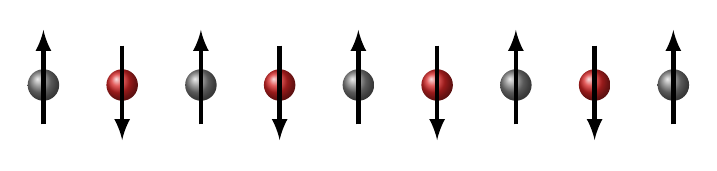
\begin{tikzpicture}
        \tikzstyle{balloon}=[ball color=gray];
        \tikzstyle{balloon2}=[ball color=red!70!gray];
        \foreach\x in {0,2,...,8}{
          \shade[balloon] (\x,0) circle (.2);% node[below right]{$m$};
          \draw[ultra thick,->](\x,-.5)--(\x,.7);
        }
        \foreach\x in {1,3,5,7}{
          \shade[balloon2] (\x,0) circle (.2);% node[below right]{$m$};
          \draw[ultra thick,->](\x,.5)--(\x,-.7);
        }
        
      \end{tikzpicture}\\
      Ferrimagnetic
    \end{center}
    When they do not cancel, then they can become magnets. This is called
    \textbf{ferromagnetism}:
    \begin{center}
      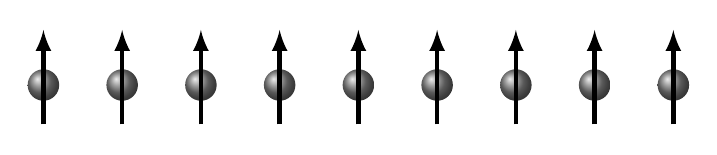
\begin{tikzpicture}
        \tikzstyle{balloon}=[ball color=gray];
        \foreach\x in {0,1,...,8}{
          \shade[balloon] (\x,0) circle (.2);% node[below right]{$m$};
          \draw[ultra thick,->](\x,-.5)--(\x,.7);
        }
      \end{tikzpicture}\\
      Ferromagnetic
    \end{center}
    Transitional elements such as iron, nickel and cobalt, and their alloys
    will exhibit ferromagnetism.
  \end{enumerate}
\end{frame}



\begin{frame}{Permanent Magnets}
  \begin{enumerate}
    \setcounter{enumi}{3}
  \item The atoms in these ferromagnetic materials are arranged in ``domains''
    wher their magnetic moment is aligned. In the presence of a strong
    external magnetic field, these domains will line up, creating a magnet.
    \begin{center}
      \pic{.6}{domain}
    \end{center}
  \end{enumerate}
\end{frame}


    
\begin{frame}{Earth}
  Earth is also a ``permanent'' magnet, with the \emph{magnetic south pole}
  located near the geographic north pole, and the \emph{magnetic north pole}
  located near the geographic south pole. The poles are tilted by
  $\approx\ang{11}$ from the spin axis.
  \begin{center}
    \pic{.5}{mearthbar}
  \end{center}
  The exact nature of Earth's magnetic field is not known, although it may be
  related to ``generator effect'' from Earth's rotation, circulating the
  outer-core fluid around.
\end{frame}



\section{Amp\`{e}re's Law}

\begin{frame}{Amp\`{e}re's Law}
  \begin{columns}
    \column{.25\textwidth}
    \pic{1}{amlaw}
    
    \column{.75\textwidth}
    Like Gauss's law is used to calculate electric fields,
    \textbf{Amp\`{e}re's law} is used to calculate the magnetic field for
    symmetric configurations:

    \eq{-.1in}{\boxed{\oint_C \vec B\cdot\dl\vec\ell=\mu_0 I_C}}
    where
    \begin{itemize}
    \item $C$ is a closed curve around a current (``Amperian loop'')
    \item $\dl\vec\ell$ is an infinitesimal length along the closed curve
    \item $I_c$ is the net current that penetrates the area bounded by $C$
    \end{itemize}
  \end{columns}
\end{frame}



\begin{frame}{Application of Amp\`{e}re's Law: Infinitely Long Wire}
  \begin{columns}
    \column{.3\textwidth}
    \pic{1}{4iM3O}

    \column{.7\textwidth}
    An \emph{infinitely} long wire must generate a magnetic field that only
    depend on radial distance. We place an Amperian loop as a circle of radius
    $r$ inside the toroid. Amp\`{e}re's law reduces to:

    \eq{-.3in}{
      \oint_C \vec B\cdot\dl\vec\ell=\mu_0 I_C
      \;\rightarrow\;
      B(2\pi r)=\mu_0 I
    }
      
    From this, we get our expression of the magnetic field from an infinitely
    long wire:
      
    \eq{-.2in}{
      B=\frac{\mu_0 I}{2\pi r}
    }
  \end{columns}
\end{frame}



\begin{frame}{Toroid}
  \begin{columns}
    \column{.3\textwidth}
    \pic1{toroid}

    {\scriptsize A toroid consists of a current-\\
      carrying wire wound around a donut-shaped core \par}
    
    \column{.7\textwidth}
    Another application of Amp\`{e}re's law is the \textbf{toroid}. This time,
    we put our loop at $a<r<b$ inside the toroid. Once again, because of
    symmetry, Amp\`{e}re's law reduces to:

    \vspace{-.35in}{\Large
      \begin{align*}
        \oint_C \vec B\cdot\dl\vec\ell &=\mu_0 I_C\\
        B(2\pi r)&=\mu_0 NI\\
        B&=\frac{\mu_0 NI}{2\pi r}
      \end{align*}
    }

    \vspace{-.15in}where $N$ is the number of times the wire is wound around
    the core
    
  \end{columns}
\end{frame}


\begin{frame}{Toroid}
  \begin{columns}
    \column{.3\textwidth}
    \pic1{toroid}

    \column{.7\textwidth}
    When the loop is placed at $r<a$, there is no enclosed
    current, and therefore the magnetic field is zero:

    \eq{-.3in}{B=0\quad\text{for}\quad r<a}

    \vspace{-.2in}When the loop is placed at $r>b$, the amount of current
    penetrating the loop is the same in both direction, i.e.\ $I_c=0$, and

    \eq{-.3in}{B=0\quad\text{for}\quad r>b}
    
    \vspace{-.1in}In fact, magnetic field \emph{only} exists inside the core,
    between $a$ and $b$.
  \end{columns}
\end{frame}




\section{Magnetic Force}

\begin{frame}{So What Does the Magnetic Field Do?}{In Classical Physics}
  \begin{columns}
    \column[t]{.3\textwidth}
    \begin{center}
      Gravitational Field $\vec g$
    \end{center}
    \begin{itemize}
    \item Generated by massive objects
    \item Affects massive objects
    \end{itemize}

    \column[t]{.3\textwidth}
    \begin{center}
      Electric Field $\vec E$
    \end{center}
    \begin{itemize}
    \item Generated by charged particles
    \item Affects charged particles
    \end{itemize}

    \column[t]{.4\textwidth}
    \begin{center}
      Magnetic Field $\vec B$
    \end{center}
    \begin{itemize}
    \item Generated by \emph{moving} charged particles
    \item Affects moving charged particles
    \end{itemize}
  \end{columns}
\end{frame}



\begin{frame}{Lorentz Force Law}
  Since a moving charge or current create both electric and magnetic fields,
  another moving charge is therefore affected by both $\vec E$ and $\vec B$.
  The total effect is given by the \textbf{Lorentz force law}:

  \eq{-.2in}{
    \boxed{\vec F=q(\vec E+\vec v\times\vec B)}
  }

  \vspace{-.1in}$\vec F_q=q\vec E$ is the electrostatic force, and
  $\vec F_m=q\vec v\times\vec B$ is the magnetic force.
  \begin{center}
    \begin{tabular}{l|c|c}
      \rowcolor{pink}
      \textbf{Quantity} & \textbf{Symbol} & \textbf{SI Unit} \\ \hline
      Total force on the moving charge & $\vec F$ & \si\newton \\
      Charge                 & $q$      & \si\coulomb \\
      Velocity of the charge & $\vec v$ & \si{\metre\per\second} \\
      Magnetic field         & $\vec B$ & \si\tesla \\
      Electric field         & $\vec E$ & \si{\newton\per\coulomb}
    \end{tabular}
  \end{center}
\end{frame}



\begin{frame}{Force on a Current-Carrying Conductor in a Magnetic Field}
  Likewise, $\vec B$ exerts a force on another current-carrying conductor.

  \eq{-.2in}{
    \boxed{\dl F_m=\vec I\dl\ell\times\vec B}
  }
  \begin{center}
    \begin{tabular}{l|c|c}
      \rowcolor{pink}
      \textbf{Quantity} & \textbf{Symbol} & \textbf{SI Unit} \\ \hline
      Magnetic force on the conductor   & $\vec F_m$ & \si\newton \\
      Electric current in the conductor & $\vec I$   & \si\ampere \\
      Length of the conductor           & $\ell$     & \si\metre \\
      Magnetic field                    & $\vec B$   & \si\tesla
    \end{tabular}
  \end{center}
\end{frame}



\begin{frame}{Magnetic Force on Two Current-Carrying Wires}
  \begin{columns}
    \column{.26\textwidth}
    \pic{1}{wirefor}

    \column{.74\textwidth}
    Two parallel current-carrying wires of length $L$ are at a distance $r$
    apart. Magnetic field at wire $2$ from current $I_1$ has constant strength
    along the wire, given by:

    \eq{-.2in}{
      B=\frac{\mu_0I_1}{2\pi r}
    }

    The force of $B$ on $I_2$ is:

    \eq{-.3in}{
      F=I_2LB=\frac{\mu_0I_1I_2L}{2\pi r}
      \;\rightarrow\;
      \boxed{\frac{F}{L}=\frac{\mu_0I_1I_2}{2\pi r}}
    }

    \vspace{-.1in}$I_1$ also exerts the same force on $I_2$, pulling the wires
    toward each other. (We should expect this because of third law of motion.)
  \end{columns}
\end{frame}



\begin{frame}{Circular Motion Caused by a Magnetic Field}
  When a charged particle enters a magnetic field at right angle\ldots
  \begin{itemize}
  \item Magnetic force $\vec F_m$ perpendicular to both velocity $\vec v$ and
    magnetic field $\vec B$.
  \item Results in circular motion
  \end{itemize}
  Centripetal force $\vec F_c$ is provided by the magnetic force $\vec F_m$.
  Equating the two expressions:

  \eq{-.2in}{
    \frac{mv^2}r=qvB
  }
  
  We can solve for $r$ get the radius for a charge with a known
  mass, or solve for mass $m$ of a charged particle based on its radius:  

  \eq{-.2in}{
    r = \frac{mv}{qB}\quad\quad\quad m=\frac{qrB}v
  }
\end{frame}



%\section{Faraday's Law}
%
%\begin{frame}{Magnetic Flux}
%  \textbf{Question:} If a current-carrying wire can generate a magnetic field,
%  can a magnetic field affect the current in a wire?
%
%  \vspace{.3in}\textbf{Answer:} Yes, sort of\ldots
%
%  \vspace{.3in}To understand how to \emph{induce} a current by a magnetic field,
%  we need to look at fluxes again.
%\end{frame}
%
%
%\begin{frame}{Magnetic Flux}
%  \begin{columns}
%    \column{.4\textwidth}
%    \pic{1}{flux2}
%  
%    \column{.6\textwidth}
%    Magnetic flux is defined as:
%    
%    \eq{-.15in}{
%      \boxed{\Phi_m=\int\vec B\cdot\dl\vec{A}}
%    }
%    
%    where $\vec B$ is the magnetic field, and $\dl\vec{A}$ is the infinitesimal
%    area pointing \textbf{outwards}. Note that magnetic flux can also be
%    expressed as:
%
%    \eq{-.2in}{
%      \boxed{\Phi_m=\int\vec B\cdot\hat n\dl A}
%    }
%
%    where $\hat n$ is the outward normal direction
%  \end{columns}
%\end{frame}
%
%
%
%\begin{frame}{Magnetic Flux Over a Closed Surface}
%  The unit for magnetic flux is a ``weber'' (\si{\weber}), in honor of German
%  physicist Wilhelm Weber, who invented the electromagnetic telegraph with Carl
%  Gauss. The unit is defined as:
%
%  \eq{-.25in}{\SI1\weber=\SI1{\tesla.\metre\squared}}
%  
%  \vspace{-.2in}The magnetic flux over a closed surface is always zero
%  (\textbf{Gauss's law for magnetism}):
%
%  \eq{-.2in}{
%    \boxed{\oint\vec B\cdot\dl\vec{A}=0}
%  }
%
%  Since magnetic field lines only exist as a loop, that means there should be
%  equal amount of ``flux'' flowing out of a closed surface as entering the
%  surface.
%\end{frame}
%
%
%%\begin{frame}{Magnetic Flux}
%%  \begin{center}
%%    \pic{.4}{flux2}
%%  \end{center}
%%
%%  
%%
%%  \vspace{-.15in}Not surprisingly, the magnetic flux is defined similar to
%%  electric flux:
%%  
%%  \eq{-.2in}{
%%    \boxed{\Phi_\mathrm{magnetic}=\int\vec B\cdot d\vec{A}}
%%  }
%%
%%  where $\vec B$ is the magnetic field, and $d\vec{A}$ is the infinitesimal area
%%  with its direction point outward.
%%\end{frame}
%%
%%\begin{frame}
%%  \frametitle{Magnetic Flux Over a Closed Surface}
%%
%%  The magnetic flux over a closed surface is always zero:
%%
%%  \eq{-.2in}{
%%    \boxed{\oint\vec B\cdot d\vec{A}=0}
%%  }
%%
%%  Since magnetic field exists in a loop only, what every flux that leaves the
%%  surface has to eventually come back.
%%\end{frame}
%
%
%\begin{frame}{Changing Magnetic Flux}
%  Changes to magnetic flux can be due to a number of reasons:
%  \begin{enumerate}
%  \item\textbf{Changing magnetic field}\ldots if the magnetic field is created
%    by a time-dependent source (e.g.\ alternating current)
%  \item\textbf{Changing orientation of magnetic field} either because the
%    surface area is moving relative to the magnetic field.
%  \item\textbf{Changing area} the surface area from which the flux is
%    calculated is changing.
%  \end{enumerate}
%\end{frame}
%
%
%\begin{frame}{When Magnetic Flux is Changing}
%  \begin{itemize}
%  \item When the magnetic flux $\Phi_m$ is changing, an electromotive force
%    (\emph{emf}, $\mathcal{E}$) is created in the wire.
%  \item Unlike in a circuit, where the \emph{emf} is concentrated at the
%    terminals of the battery, the induced \emph{emf} is spread across the
%    entire wire.
%  \end{itemize}
%  \begin{columns}
%    \column{.3\textwidth}
%    \begin{center}
%      \begin{tikzpicture}[scale=.35]
%        \foreach \xx in {-4.5,-3,...,4.5}{
%          \foreach \yy in {-4.5,-3,...,4.5}{
%            \node at (\xx,\yy)
%                  {\footnotesize\textcolor{green!80!black}{$\times$}};
%          }
%        }
%        \draw[gray,ultra thick](0,0) circle(2.9);
%        \draw[->,rotate=45](0,0)--(2.9,0) node[midway,left]{\footnotesize $r$};
%        \foreach \x in {0,90,...,360} {
%          \begin{scope}[rotate=\x]
%            \draw[ultra thick,red!80!black,->](2.9,0)--(2.9,2.5)
%            node[pos=0,above left]{$\vec{E}$};
%          \end{scope}
%        }
%      \end{tikzpicture}
%    \end{center}
%    
%    \column{.7\textwidth}
%    \begin{itemize}
%    \item Since \emph{emf} is work per unit charge, that means that there is an
%      electric field inside the wire to move the charges.
%    \item In this example:
%      \begin{itemize}
%      \item Magnetic field $\vec B$ into the page
%      \item The direction of the electric field $\vec{E}$ corresponds to an
%        \emph{increase} in magnetic flux
%      \end{itemize}
%    \end{itemize}
%  \end{columns}
%\end{frame}
%
%
%\begin{frame}{Faraday's Law}
%  Faraday's law states that the rate of change of magnetic flux produces an
%  electromotive force:
%
%  \eq{-.2in}{
%    \boxed{
%      \mathcal{E}=\oint\vec{E}\cdot\dl\vec{l}={\color{red}{-}}
%      \diff{\Phi}t
%    }
%  }
%  
%  The negative sign {\textcolor{red}{highlighted in red}} is the result of
%  Lenz's law, which is related to the conservation energy
%\end{frame}
%
%
%
%\begin{frame}{AC Generators}
%  A simple AC (alternating current) generator makes use of the fact that a 
%  coil rotating against a fixed magnetic field has a changing flux.
%  \begin{center}
%    \pic{.45}{generator}
%  \end{center}
%  Let's say the permanent magnets produce a uniform magnetic field $B$, and the
%  coil between them has $N$ turns, and an area $A$. Now let's say that the coil
%  is rotating with an angular frequency $\omega$.
%\end{frame}
%
%
%
%\begin{frame}{AC Generators}
%  \begin{columns}
%    \column{.35\textwidth}
%    \pic{1}{generator}
%
%    \column{.65\textwidth}
%    When the coil is turning, the angle between the coil and the magnetic field
%    is:
%    
%    \eq{-.2in}{
%      \theta=\omega t+\delta
%    } 
%
%    \vspace{-.1in}where $\delta$ is the initial angle. The magnetic flux
%    through the coil is given by:
%    
%    \vspace{-.4in}{\Large
%      \begin{align*}
%        \Phi&=NBA\cos\theta\\
%        &=NBA\cos(\omega t+\delta)
%      \end{align*}
%    }
%    
%    \vspace{-.3in}as the coil turns.
%  \end{columns}
%\end{frame}
%
%
%
%\begin{frame}{AC Generators}
%  \begin{columns}
%    \column{.33\textwidth}
%    \pic{1.05}{generator}
%
%    \column{.67\textwidth}  
%    The electromotive force \emph{emf} produced is therefore the rate of change
%    of the magnetic flux:
%
%    \vspace{-.3in}{\Large
%      \begin{align*}
%        \mathcal{E} &=-\diff{\Phi_m}t\\
%        &=\underbracket{NBA\omega}_{\mathcal{E}_\text{max}}\sin(\omega t+\delta)
%      \end{align*}
%    }
%  \end{columns}
%\end{frame}
%
%
%
%%\begin{frame}{AC Generators}
%%  \begin{columns}
%%    \column{.35\textwidth}
%%    \pic{1}{generator}
%%
%%    \column{.65\textwidth}
%%    We commonly write it this way instead:
%%    
%%    \eq{-.25in}{\mathcal{E}=\mathcal{E}_{\textrm{max}}\sin(\omega t+\delta)}
%%    
%%    \vspace{-.2in}where
%%
%%    \eq{-.25in}{
%%      \mathcal{E}_{\textrm{max}}=NBA\omega
%%    }
%%  \end{columns}
%%\end{frame}
%
%
%
%\begin{frame}{Motional EMF}
%  {What happens when I slide the rod to the right?}
%  \begin{columns}
%    \column{.45\textwidth}
%    \pic{1}{motional-emf-1}
%
%    \column{.55\textwidth}
%    When sliding the rod to the right with speed $v$, the magnetic flux through
%    the loop (and its rate of change) is:
%
%    \vspace{-.4in}{\Large
%      \begin{align*}
%        \Phi&=BA=B\ell x\\
%        \diff{\Phi}r &= B\ell\diff xt=\boxed{B\ell v=\mathcal{E}}
%      \end{align*}
%    }
%    
%    We can use the Lorentz force law on the charges on the rod to find the
%    direction of the current $I$.
%  \end{columns}
%\end{frame}
%
%
%
%\begin{frame}{Motional EMF}{What happens when I slide the rod to the right?}
%  \begin{columns}
%    \column{.22\textwidth}
%    \begin{tikzpicture}[scale=1.5]
%      \draw[thick](1.5,0) to[battery1,l_=$\mathcal{E}$] (1.5,1.5)--(0,1.5)
%      to[R,l_=$R$] (0,0)--(1.5,0);
%    \end{tikzpicture}
%    
%    \column{.78\textwidth}
%    \begin{itemize}
%    \item An equivalent circuit is shown on the left
%    \item The amount of current can be found using Ohm's law: $V=IR$
%    \item Note that the ``motional emf'' produced is spread over the entire
%      circuit
%      \begin{itemize}
%      \item In constrast, in a voltaic cell (or battery), the \emph{emf} is
%        concentrated between the two terminals.
%      \end{itemize}
%    \end{itemize}
%  \end{columns}
%\end{frame}
%
%
%
%\section{Lenz's Law}
%
%\begin{frame}{Lenz's Law}
%  Something very interesting happens when the current starts running on the
%  wire.
%  \begin{center}
%    \pic{.35}{motional-emf-2}
%  \end{center}
%  It produces an ``induced magnetic field'' out of the page, in the opposite
%  direction as the field that generated the current in the first place.
%\end{frame}
%
%
%
%\begin{frame}{Lenz's Law}
%  \begin{center}
%    \fbox{
%      \begin{minipage}{.7\textwidth}
%        \textbf{LENZ'S LAW}\\
%        The induced \emph{emf} and induced current are in such are
%        direction as to oppose the change that produces them
%      \end{minipage}
%    }
%  \end{center}
%
%  \vspace{.2in}So basically, the conservation of energy
%\end{frame}
%
%
%
%\section{Inductance}
%
%\begin{frame}{Back \emph{emf}}
%  Consider a very simple circuit consisting of a voltage source and a coil
%  \begin{center}
%    \begin{tikzpicture}[american voltages,scale=1.3]
%      \draw[thick](0,0) to[battery1,l=$\mathcal{E}$] (0,1.5)
%      to[short,-*](.5,1.5);
%      \draw[thick](.55,1.7) to[short,*-*](1,1.5)--(1.5,1.5)
%      to[L] (1.5,0)--(0,0);
%    \end{tikzpicture}
%  \end{center}
%  \begin{itemize}
%  \item When the switch is closed and current begins to flow, the coil
%    begins to generate a magnetic flux inside
%  \item As the current changes (initially increasing with time), it
%    self-induces a ``back \emph{emf}'' that opposes the change in current
%  \item A current can't jump from zero to some value (or from some value to
%    zero) instantaneously
%  \end{itemize}
%\end{frame}
%
%
%
%\begin{frame}{Back \emph{emf}}
%  \begin{center}
%    \begin{tikzpicture}[american voltages,scale=1.3]
%      \draw[thick](0,0) to[battery1,l=$\mathcal{E}$] (0,1.5)
%      to[short,-*](.5,1.5);
%      \draw[thick](.55,1.7) to[short,*-*](1,1.5)--(1.5,1.5)
%      to[L] (1.5,0)--(0,0);
%    \end{tikzpicture}
%  \end{center}
%  \begin{itemize}
%  \item Breaking the circuit causes the magnetic flux to change very rapidly
%  \item The rapid change of $\Phi_m$ creates a large induced back \emph{emf}
%    that is proportional to the time rate of change of magnetic flux
%    $\Phi_m'(t)$
%  \item The back \emph{emf} creates a large voltage drop across the switch
%  \item Large voltage across two metal contact produces a very strong electric
%    field--strong enough to tear electrons away from air molecules
%    (``dielectric breakdown'')
%  \item Air conducts electricity in the form of a ``spark''
%  \end{itemize}
%\end{frame}
%
%
%
%\begin{frame}{Self Inductance}
%  A solenoid carrying a current generates a magnetic field $B$; its magnitude at
%  the core is proportional to the current $I$:
%
%  \eq{-.2in}{
%    B=\left[\frac{\mu_0N}\ell\right]I
%  }
%
%  Since $\vec B\propto I$, the magnetic flux through the core of the solenoid
%  (really $\Phi_m=NBA$, where $A$ is the cross-sectional area of the solenoid
%  and $N$ is the number of coils) is therefore also proportional to $I$, i.e.
%
%  \eq{-.2in}{
%    \boxed{\Phi_m=LI}
%  }
%
%  where $L$ is the called the \textbf{self inductance} of the coil.
%\end{frame}
%
%
%
%\begin{frame}{Self Inductance}
%  For a solenoid, we can see that the self inductance is given by:
%
%  \eq{-.2in}{
%    \boxed{L=\frac{\Phi_m}{I}=\mu_0 n^2A\ell}
%  }
%
%  \begin{center}
%    \begin{tabular}{l|c|c}
%      \rowcolor{pink}
%      \textbf{Quantity} & \textbf{Symbol} & \textbf{SI Unit} \\ \hline
%      Self inductance                    & $L$     & \si{\henry}\\
%      Vacuum permeability                & $\mu_0$ & \si{T.m/A} \\
%      Number of coils per unit length    & $n$     & \si{\ampere} \\
%      Cross-section area of the solenoid & $A$     & \si{\metre^2} \\
%      Length of the solenoid             & $\ell$  & \si{\metre}
%    \end{tabular}
%  \end{center}
%  Note that $A\ell$ is the \emph{enclosed volume} of the solenoid.
%\end{frame}
%
%
%
%\begin{frame}{Self Inductance and Induced EMF}
%  If the current changes, the magnetic flux changes as well, therefore inducing
%  an electromotive force in the circuit According Faraday's law:
%
%  \eq{-.1in}{
%    \boxed{\mathcal{E}=-\diff {\Phi_m}t=-L\diff It}
%  }
%
%  The self-induced \emph{emf} is proportional to the rate of change of current
%\end{frame}
%
%
%
%\begin{frame}{Magnetic Energy}
%  At any instant, the magnitude of the induced emf is
%
%  \eq{-.2in}{
%    \mathcal{E}=L\diff It
%  }
%  so the power absorbed by the inductor is
%
%  \eq{-.2in}{
%    P(t)=\mathcal{E}I=LI\diff It
%  }
%
%  Integrating in time gives the magnetic (potential) energy that is stored in
%  the magnetic field:
%
%  \eq{-.2in}{
%    U_m
%    =\int_0^t P(\tau)\dl\tau
%    =L \int I\diff I\tau \dl\tau
%    =L \int_0^I I\dl I=\frac12LI^2
%  }
%\end{frame}
%
%
%
%\begin{frame}{Magnetic Energy}
%  Just as a capacitor stores energy in its electric field, an inductor coil
%  carrying a current $I$ stores energy in its magnetic field, given by:
%
%  \eq{-.2in}{
%    \boxed{U_m=\frac12LI^2}
%  }
%
%  We can also define a \textbf{magnetic energy density}:
%
%  \eq{-.2in}{
%    \boxed{\eta_m=\frac{B^2}{2\mu_0}}
%  }
%\end{frame}
%
%
%%\section{LC Circuit}
%%\begin{frame}
%%  \frametitle{LC Circuit}
%%  The final type of circuit that we will study in AP Physics is the LC
%%  circuit. In its simplest form, the circuit has an inductor and capacitor
%%  connected in series:
%%  \begin{center}
%%    \begin{tikzpicture}[american voltages,scale=1.2]
%%      \draw[thick](0,0) to[L=$L$] (0,2)--(2,2) to[C=$C$] (2,0)--(0,0);
%%    \end{tikzpicture}
%%  \end{center}
%%  We apply the Kirchkoff's voltage law:
%%  
%%  \eq{-.2in}{
%%    -V_L-V_C=0
%%    \quad\rightarrow\quad
%%    L\frac{dI}{dt}+\frac{Q}{C}=0
%%  }
%%\end{frame}
%%
%%\begin{frame}
%%  \frametitle{LC Circuits}
%%  Since both terms are continuously differentiable, we can differentiate both
%%  sides of the equation, which gives:
%%
%%  \eq{-.2in}{
%%    L\frac{d^2I}{dt^2}+\frac{1}{C}\underbrace{\frac{dQ}{dt}}_I=0
%%  }
%%
%%  In fact, the above equation is one that we have studied many topics ago:
%%
%%  \eq{-.2in}{
%%    \frac{d^2I}{dt^2}+\frac{1}{LC}I=0
%%  }
%%
%%  This is a second-order ordinary differential equation, and the solution is
%%  the simple harmonic motion.
%%\end{frame}
%%
%%
%%\begin{frame}
%%  \frametitle{LC Circuit}
%%  The current inside of an LC circuit is given by:
%%
%%  \eq{-.2in}{
%%    I(t)=I_0\sin(\omega t + \varphi)\quad\text{where}\quad
%%    \omega=\frac{1}{\sqrt{LC}}
%%  }
%%\end{frame}
%%
\end{document}
